\documentclass[conference]{IEEEtran}
\IEEEoverridecommandlockouts
% The preceding line is only needed to identify funding in the first footnote. If that is unneeded, please comment it out.
\usepackage{cite}
\usepackage{amsmath,amssymb,amsfonts}
\usepackage{algorithmic}
\usepackage{graphicx}
\usepackage{textcomp}
\usepackage{xcolor}
\usepackage[utf8]{inputenc}
\def\BibTeX{{\rm B\kern-.05em{\sc i\kern-.025em b}\kern-.08em
    T\kern-.1667em\lower.7ex\hbox{E}\kern-.125emX}}
\begin{document}


\title{Wake alarm - Using a react-native client in combination with a rust backend.}

\author{\IEEEauthorblockN{1\textsuperscript{st} Maksim Sandybekov}
\IEEEauthorblockA{\textit{computer science - autonomouse systems)} \\
\textit{HTWG Konstanz}\\
Konstaz, Germany \\
maksim.sandybekov@live.de}
\and
\IEEEauthorblockN{2\textsuperscript{nd} Benjamin Bäumler}
\IEEEauthorblockA{\textit{computer science - autonomouse systems} \\
\textit{HTWG Konstanz}\\
Konstanz, Germany \\
be391bae@htwg-konstanz.de}
}

\maketitle

\begin{abstract}


\end{abstract}

\begin{IEEEkeywords}
rust, react-native, redux, redux-saga, light, alarm, smart-light
\end{IEEEkeywords}

% Motivation, why are we doing the likes
\section{Introduction}
The quality and duration of sleep affects the health and well being of individuals.
Additionally sleep plays a major role in consolidation of memory \cite{Rauchs2005} therefore it is essential for learning process.
Looking at studies on sleep deprevation and disorders it becomes clear that a poor sleep can cause an decrease in both
mental and physical performance. \cite{Mirghani2015a, Antunes2017a} Leading up to variouse physical and mental
diseases for example type-2 diabities, anxiety and increased depression. Especially students represent a group that 
is likely to suffer sever sleep deprevation. In an conducted study 46\% of 546 students rated their sleep as failry bad up to 
very bad. Furthermore 33\% of participants reported $\leq$ 7 h of sleep on study days with an average of 6.55 h. \cite{Norbury2019a}

The research surrounding the impact of light on the human circadian clock thereby revelead an relationship between illuminance and
alertness in human beings. \cite{DuffyJeanne2009a} In addition further research uncovered a link between exposure to more intense
light and the feeling of vitality during daytime and everyday situations. \cite{Smolders2014a}

These insights suggests a system that utilizes the effects of light on the human body to improve alertness and mental as well as
pyhsical performance during the day. Using these mechanisms within the context of circadian stimulation and sleep, different
fields of application become obviouse.

While technological development proceeds there are already attempts utilizing current innovations to harness prior introduced 
positive effects. One such attempt are wake lights that simulate the sunrise. A study investigating effects on the human body
concludes that simulation of the dawn significantly improves performance on attention- and motor-based tasks/skills during the day.
\cite{Gabel2015a}

This paper proposes an application implementing functionality to utilize previousely introduced advances in research 
concerning the effects of light on the human body. The application enables a user to obtain controll over a smart lamp
to regulate the illumination, color. An additional system for scheduling of illumination facilitates the simulation of sunrises.

\section{State of the art}
Currently there is a broad range of available commercial products depicted as smart lamps. But surely there needs to be done a
distinction, because these devices often differ in their capabilities and technological stacks. 


% Approach
\section{Proposed approach}
To enable users to make full use of a lightning system, there is a need for the right control mechanisms to be in place.
Basic operations a user may take are activation/deactivation, change of color and brightness of the lamp. The context of use can be broadend 
by adding the possibility to schedule the activation of the light. This operation enables the use as a visual alarm clock or an automated
lighting system. 

We propose a distribution into client and server, already seen in different application. The client resembles a mobile application
offering functionality. On the opposite the server represents the device itself communicating with the client to offer an interface for
interaction with the light.

The communication between both instances happens through a wireless-network. As we are only interesseted to visualize the possibilitiy 
to develop a universally usable lighting system, a security layer will not be defined but should be in a production build. 


\subsection{Architecture}
On an architectural level the application firstly is divide into client and server.

\begin{figure}
    \centering
    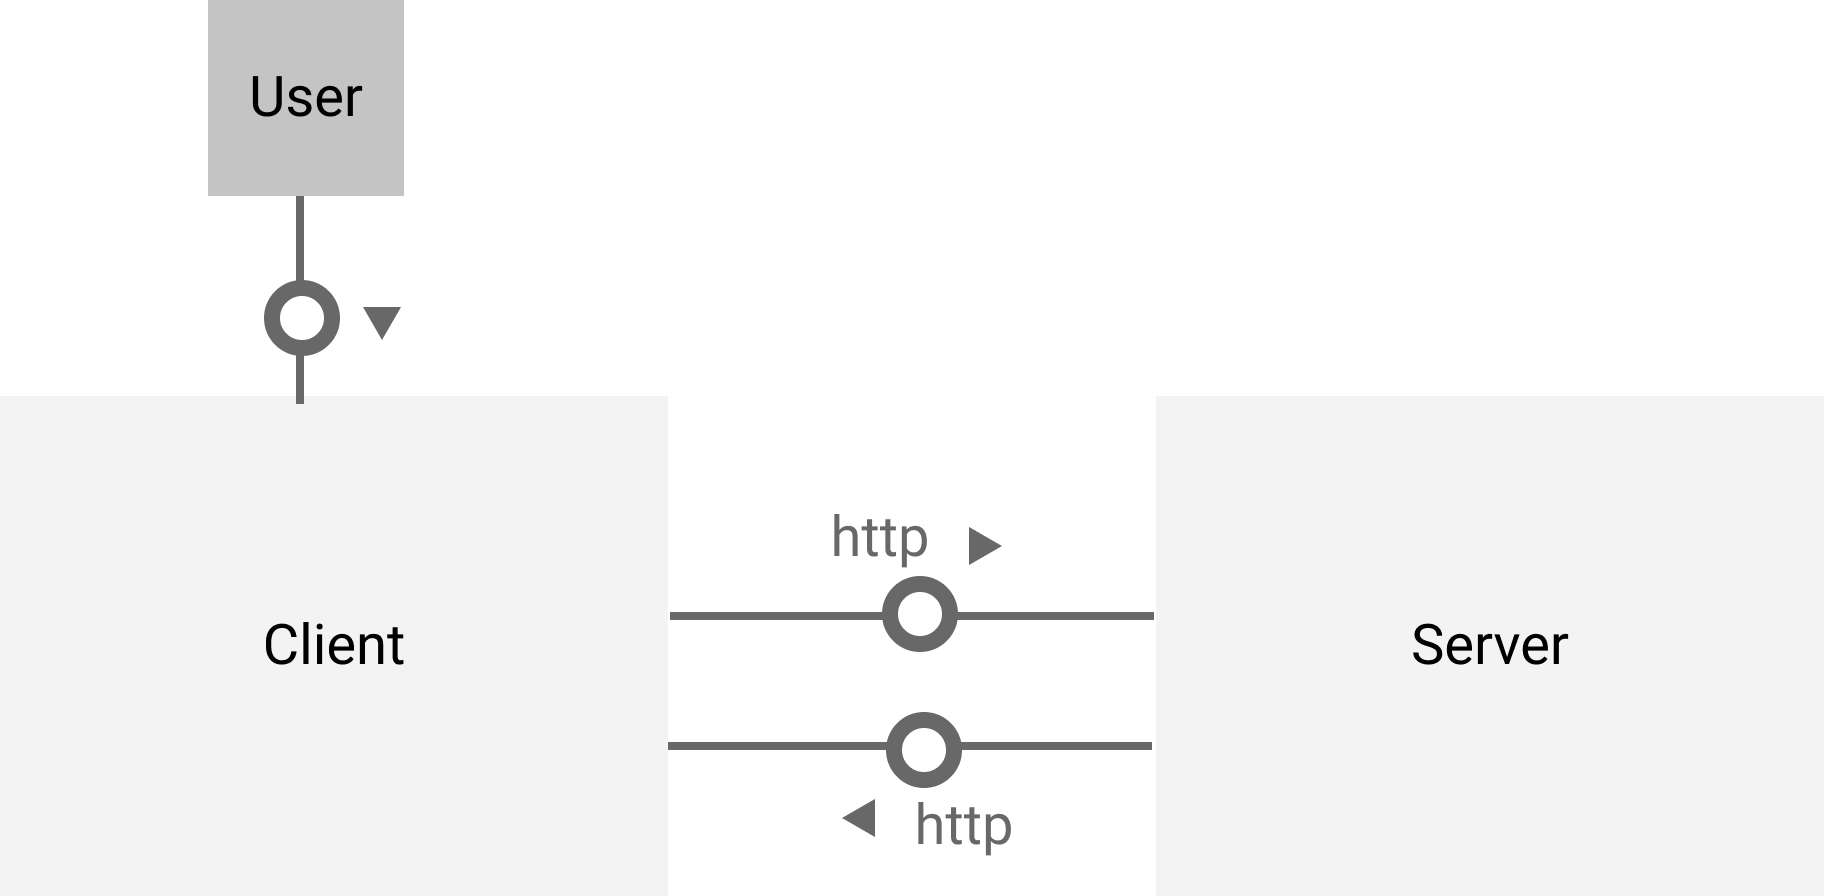
\includegraphics[width=0.4\textwidth]{top_level_architecture}
    \caption{Top level architecture}
\end{figure}



\begin{figure}
    \centering
    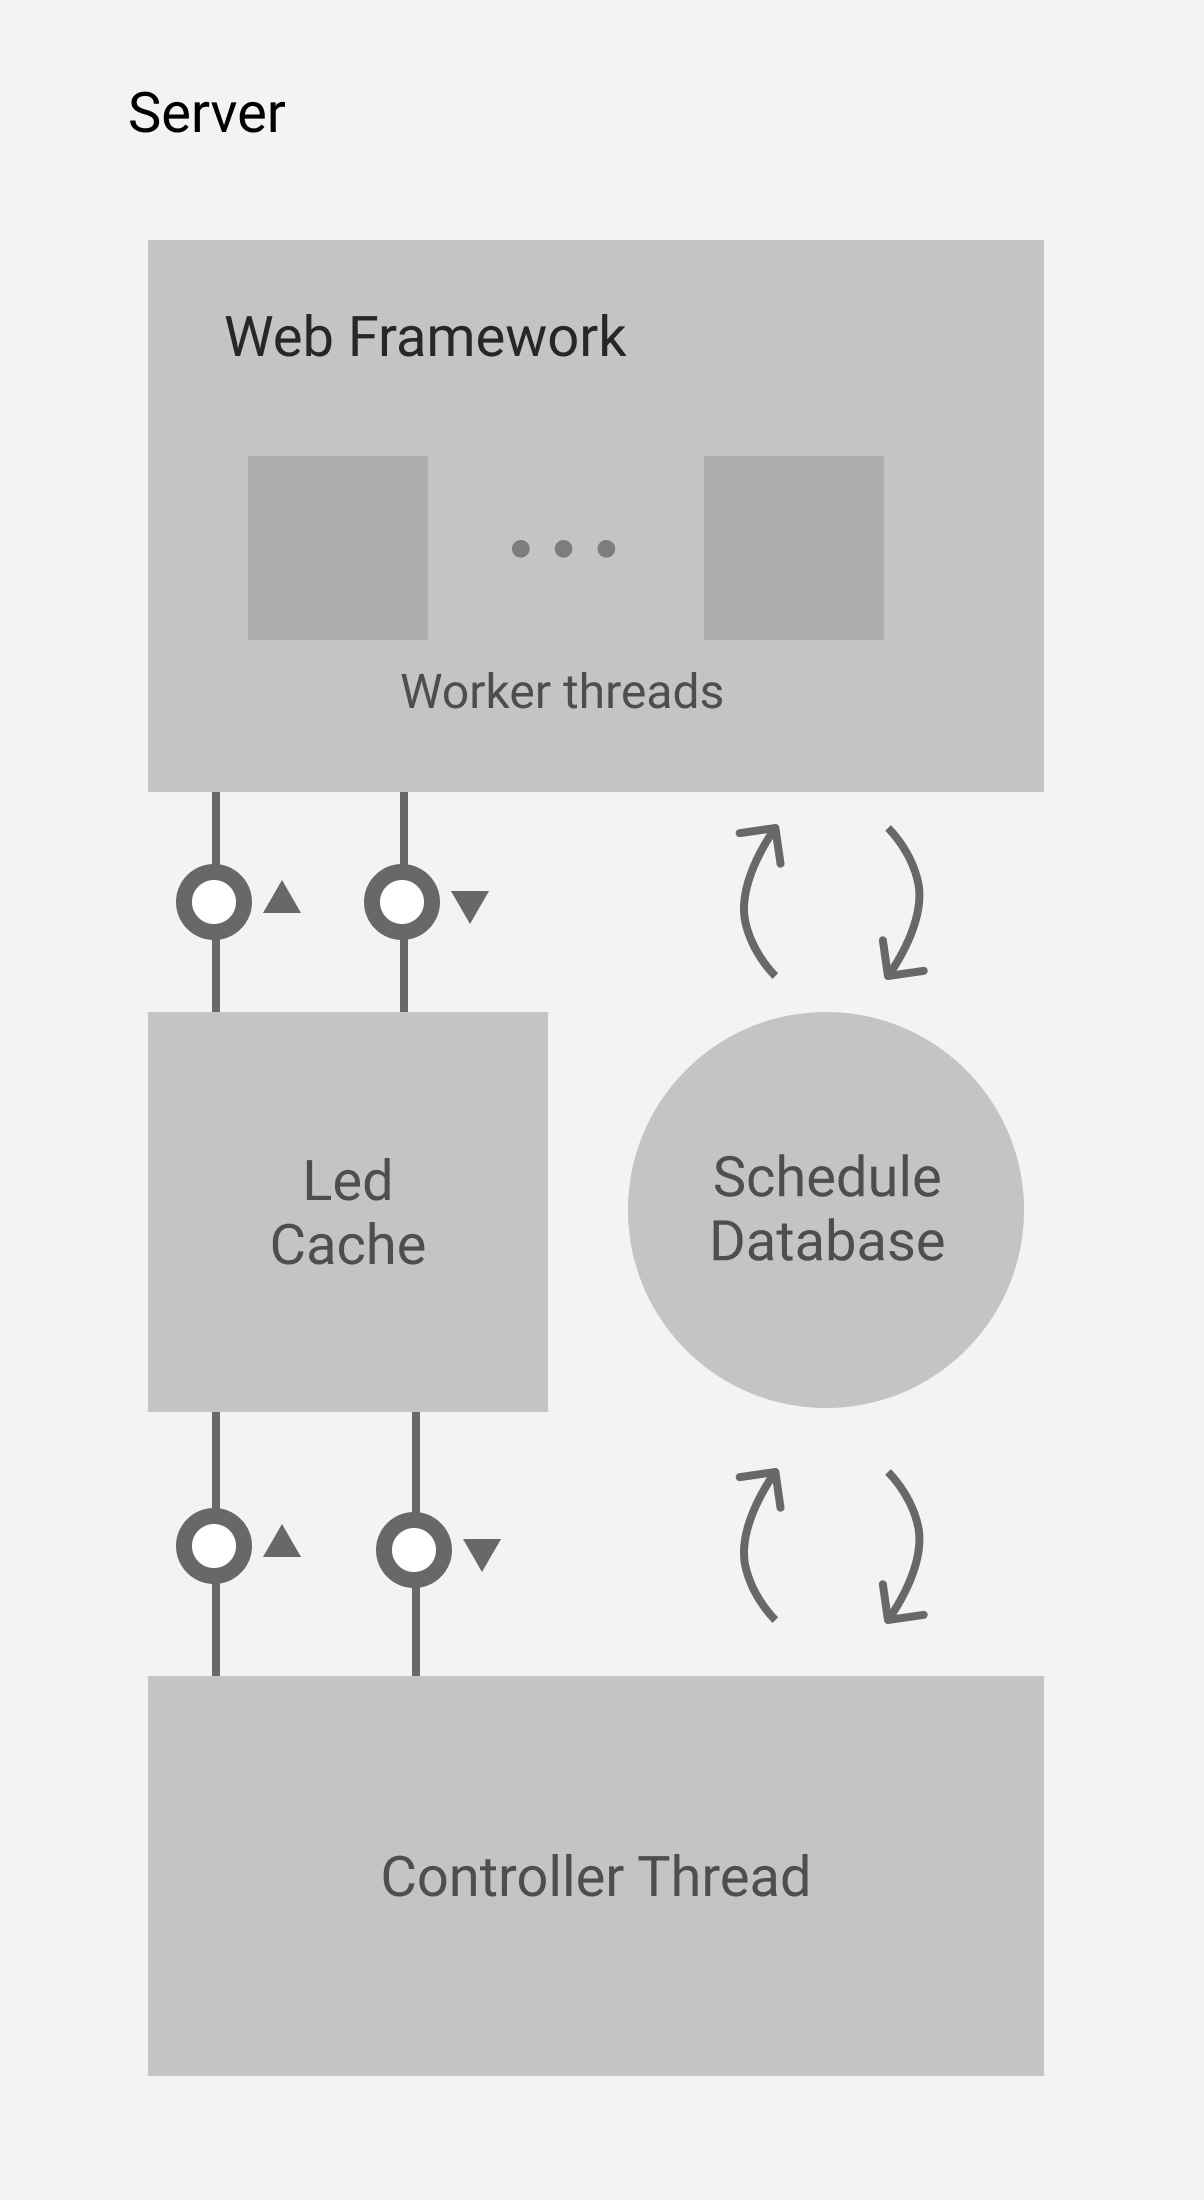
\includegraphics[width=0.4\textwidth]{server_architecture}
    \caption{Server architecture}
\end{figure}



\begin{figure}
    \centering
    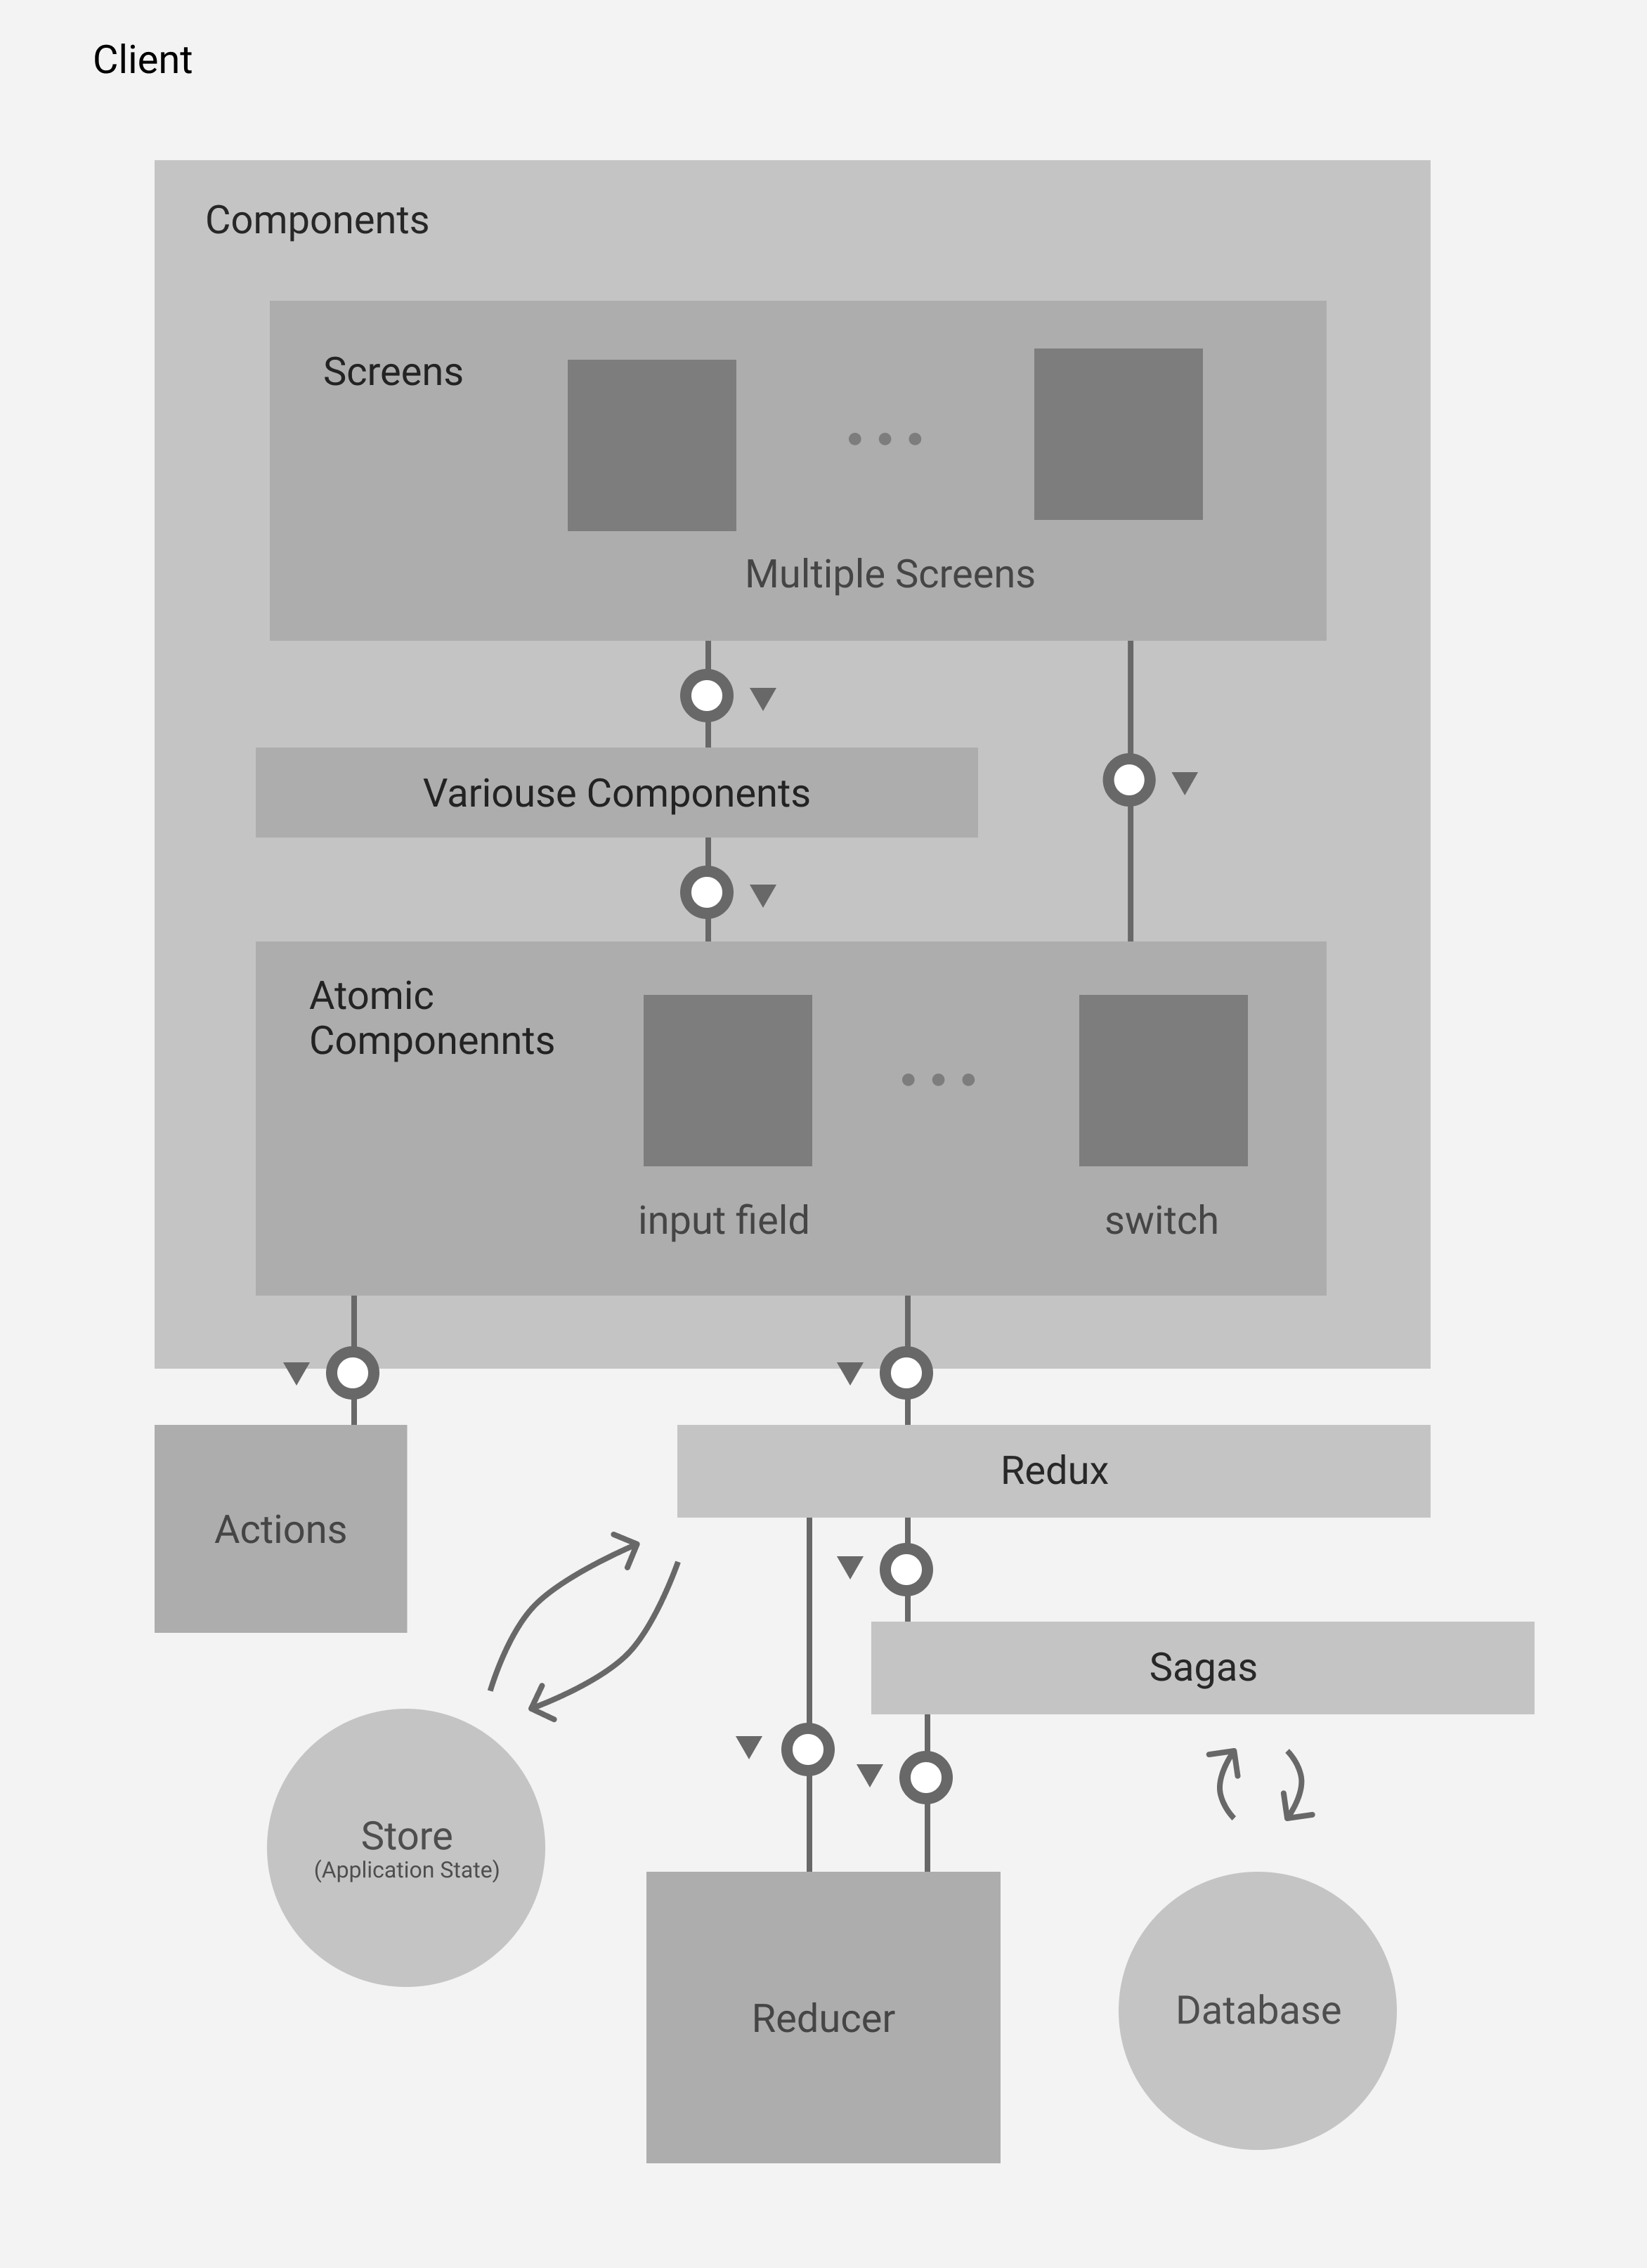
\includegraphics[width=0.4\textwidth]{client_architecture}
    \caption{Client architecture}
\end{figure}


\subsection{Client}
% UI Compoenents in correlation with the basic operations
% realization on technical level
The client is purely written in react-native/javascript. This technologie enables cross-plattform development of mobile applications while offering
rather quick development cycles. Apart from programmatical differences this library requires another mindset than native development.
Compared to other technolgies the user-interface consists of so called components each of which is made up of native elements. The developed components
may be reused and composed to create new components. In addition it is possible to pass properties to a component. These are compareable with xml
attributes, inside the component itself they can be accessed as an object. 

In our case we divided the visuals in atomic components representing for example input fields and buttons. Subsequently building
heavier components compounded out of this smaller parts. At the top most level, we simply have screen components that consist of other components 
themselves. Each of these screens providing a different functionality to the user. Following are the main screens listed.

\begin{itemize}
    \item \textbf{DeviceSetupScreen:} setting up a new device
    \item \textbf{LightScreen:} activate/deactivate light and set brightness
    \item \textbf{ColorSelectionScreen:} change color of the led
    \item \textbf{scheduleScreen:} schedule led activation 
\end{itemize}
\vspace{5pt}

% as there can be identified different parts of the application
% divide into part (presentation layer (components), store (similar to model), )

\subsubsection{Navigation}
As the application consists of mutliple screens and react-native doesen't provide a native possibility to navigate between screens an additional
library is needed. At present there are mainly two libraries available react-native-navigation and react-navigation. These libraries mainly differ
in the interface provided for navigation and their performance. The selection in our case was of agnostic nature, prefering the one with a
shallower learning curve. 

\subsubsection{State-management}
While a component is able to maintain state, looking at compound components it may appear that the same state needs to be managed at different
spots. A far better practice for this occurence involves the usage of an additional library designed especially for state-management. As this
question often arises in javascript applications, different attempts have been made to solve this issue. Many of which is the redux library,
which we selected because it is well documented and easiliy integrateable with react-native. Representing a predictable-state container the redux
library centralizes state in the so called store. 

For a component to access the state it first must connect to the store. Afterwards a mapping must be defined of state variables onto the property 
object of that specific component. To change state variables actions needed to defined which are getting dispatch by redux to reducers. While actions
represent simple javascript functions returning an object with a minimum a type field and additional payload, the reducers are listenting for
different action types and using the payload to transfer the old to the new state. 

\subsubsection{Communicaton/side effects}
For the communication with the server we limited ourself the http protocol. As there is no network discovery implemented the user needs to know the
IP address of the server he wants to connect to. To ease the task at hand and keep a clear sepeartion from the presentation layer we use the 
redux-saga library. Like the name suggest this library builds upon redux. This library mainly listens to dispatched actions and triggers generators
which execute side effects such as http calls to the server or database writes and reads. These in return can dispatch actions themselves.

The applications uses this functionality to aquire the current schedules from the server, as well as the current state of the device for example the
led brightness and color of the led. These values are stored in the store of the device.



\subsection{Server}

The main tasks of the server is to communicate with clients and to actually drive a led strip or any other kind of light source. This is realised through two main components a web framework to serve a REST-api that is used to communicate with clients and a controller running in a seperate thread, containing all the logic and managing the light source.

\subsubsection{Concurrency}

The execution flow of the controller and the web framework should be independent. We archive that by utilizing threads. Using Rust allows us to confidently write multithreaded applications\cite{rust:con}, by preventing data races in the first place and with its provided concurrency primitives.
Message passing is used to communicate between the web framework and the controller. The controller loop will check each time at the beginning if it received a message from the web framework and will handle it. Currently the controller handles five different messages:
\begin{itemize}
    \item GetData:
    The web framework needs the current led data to response to a request.
    \item UpdateOn, UpdateColor and UpdateBrightness:
    The controller should use the new provided value and use it and in case a schedule is running it will be stopped.
    \item DatabaseChanged:
    The web framework modified the database containing all schedules, the controller should check if the modification is relevant for it.
\end{itemize}

The web framework only expects two messages:
\begin{itemize}
    \item DataChanged: 
    Some data changed since the last time the web framework updated its copy and should update it again.
    \item DataDump:
    Contains all data relevant to led status. Web framework needs to actively request it with \texttt{GetData}. This is done because the controller can't know when it will need the data and sending it each time some data changed may overflow the message queue, because it gets only checked when an api request is received.
\end{itemize}

The web framework doesn't communicate with the controller directly and uses instead a \texttt{LedCache}. Through it the web framework can access the current values of the light source or change them. The \texttt{LedCache} makes sure that it only communicates with the controller thread when necessary.


\subsubsection{Light Sources}

The server can support different kinds of light sources, as long as it implements the \texttt{LedControls} trait. Only one implementation 
of the trait can be used at the same time tho. But it is possible that a specific implementation controls multiple hardware lights.
At the current time there are only two implementations that can be used as light sources:

\begin{itemize}
    \item LedStrip
    
    Controls a 4-pin led strip with a 12v pin and one pin for each color(red, green,blue). This cannot be driven directly by the
    Raspberry Pi and therefore we need to use a extra curcuit board\cite{rpiled} for it. The circuit board allows us to controll each
    color seperatly by driving the gate pin of a MOSFET's respectivly. We will use the pigpio Daemon\cite{pigpiod} for this, because we 
    need 3 PWM pins for this and currently available gpio libraries for Rust only over up to 2 PWM pins.
    
    % TODO: add picture
    **picture of circuit board**

    \item MocLedStrip
    
    This is used only for testing. It allows us to verify the logic of the led controller without driving any GPIO's of the Raspberry Pi 
    and also allows us to run the server on amd64 architecure for testing purposes.
\end{itemize}



\section{Results}


\section{Conclusion}


\section{Further work}

% Network discovery
%  


% Add Links into bib file
% \begin{thebibliography}{00}
% \bibitem{b0} Raspberry Pi \& RGB LED-Strips How to control a RGB LED-Strip with a Raspberry Pi By David Ordnung - https://dordnung.de/raspberrypi-ledstrip/
% \bibitem{b1} pigpio Daemon - http://abyz.me.uk/rpi/pigpio/pigpiod.html
% \bibitem{a0} Smart LED Lamp with Bluetooth Speaker and Clock - https://store.earlham.edu/smart-led-lamp-bluetooth-speaker-and-clock
% \bibitem{a1} 
% \end{thebibliography}

\bibliographystyle{amsplain}
\bibliography{moco}


% \vspace{12pt}

\end{document}
